\chapter{Introduction}
The \ac{IOT} is enabling communication among huge numbers of diverse low power devices.  
According to an estimate by Ericsson \cite{noauthor_internet_2017}, there will be 20 billion connected \ac{IOT} devices by 2023.
Modern communication protocols need to evolve rapidly to enable reliable connection among these devices.
The communication needs for a field temperature sensor differs from those of an industrial controller. 
Hence, there is need for research and development of communication protocols that satisfy these diverse device communication needs. 
The evaluation of these experimental protocols is difficult because of the need of specialized radio hardware.
Simulation is widely used to evaluate these protocols but they fall short on modeling of real world performance.
\ac{sdr} devices can be a powerful platform for enabling the real-world evaluation of these protocols.\\

\ac{sdr} are flexible radio platforms where most of the communication systems functionality is designed in software. Typically, \ac{sdr} platforms have on board radio front-end equipped with wide band antennas and analog signal processing chain for tuning the carrier frequency and desired bandwidth. High speed data converters convert the incoming analog signals into the digital domain and vice-versa. In traditional radios, the digital processing chain of a wireless protocol physical layer is implemented on the same chip as the radio front-end and analog signal processing functions. \ac{sdr}, on the other hand, in host-PHY \cite{nychis_enabling_nodate} architecture transfers the converted data to a general purpose computing platform using bus transfer (USB, PCIe).  The digital processing chain is designed in software, thus allowing for flexibility in the protocol design, enabling experimentation in decoding and modulation techniques. \ac{sdr} also allows for careful analysis of RF signals as the raw sample data is made available to the host.\\

\begin{figure}[!h]
\centering
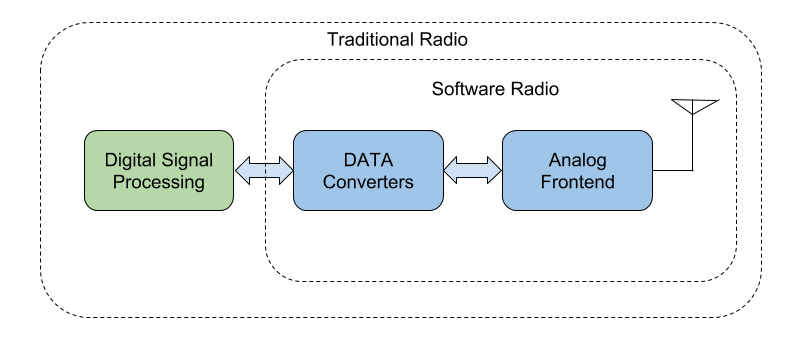
\includegraphics[width=0.75\textwidth]{Figure/SDRSystem.png}
\caption{Software Radio and Traditional Radio Architecture.}
\label{sdr_architecture}
\end{figure}


%\ac{sdr} helps to protect investments by facilitating change of protocols on already existing system. A major motivation within the commercial communications arena, is the rapid evolvement of communications standards, making software upgrades of base stations a more attractive solution than the costly replacement of base stations\cite{ulversoy_software_2010}. \ac{sdr} also opens up the possibility of Cognitive Radios, a context sensitive radio system that can adapt depending on the radio channel conditions and applications. \\

The movement of digital signal processing functions from hardware to software leads to performance issues in \ac{sdr} systems.
A fundamental challenge of \ac{sdr} system is computational horsepower, because it needs to process complex data wave-forms in a reasonable time-frame. Since \ac{sdr} involves transferring of signals and data from one system to another, this introduces considerable communication delays. Finally, general purpose processing systems introduces non-determinism in data processing and communication processes.\\


\section{Problem Context}
Wireless devices share the wireless channel with other devices. The wireless protocol \ac{mac} layer is responsible for moderating access to the wireless channel. It typically uses \ac{tdma} and \ac{csma} to allocate the use of the channel. \ac{tdma} protocols schedule the allocation of the entire channel to one of the devices for a particular time duration. This requires global time synchronization among the devices so that the devices can understand when to transmit and receive. \ac{csma}, on the other hand uses the channel on an opportunistic basis, with the devices sensing if the channel is free or not.\\

\subsection{CSMA}
As highlighted by \cite{schmid_experimental_2007}, \ac{sdr} based systems don't comply with the stringent timing constraints imposed by modern \ac{mac} protocols. Furthermore, the presence of long bus communication and processing delays create blind spots\cite{schmid_experimental_2007} in carrier sensing. In Figure \ref{blind_spots}, the \ac{sdr} system is receiving a packet being transmitted on the air medium. Since there is communication and processing delays, the \ac{cpu} of the \ac{sdr} system  receives the packet completely at $t_1$ delayed from $t_0$ when the packet transfer ends on the air medium.\\

Once the packet has been received, the system wants to let the transmitting system about the successful reception by sending the \ac{ack} packet. If it detects the medium is free using carrier sensing, it would start transmitting.
But because of the delays, it would make this decision based on past information which has been delayed by $t_1 - t_0$.
This makes the system blind towards the real time channel situation when making the decision to transmit and might lead to a collision. \\ 

\begin{figure}[!h]
\centering
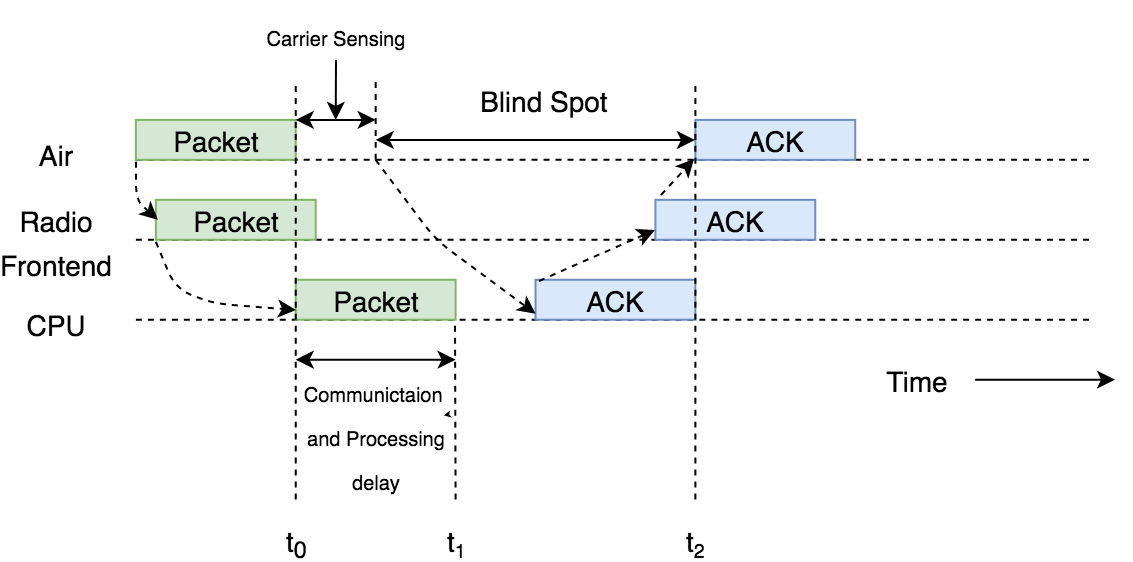
\includegraphics[width=0.6\textwidth]{Figure/BlindSpots.png}
\caption{Blind Spots Illustration(adapted from \cite{schmid_experimental_2007}).}
\label{blind_spots}
\end{figure}

Hence when designing \ac{mac} protocols, these delays needs to be taken into account to avoid collisions.
This necessitates a closer understanding of these delays and how different system parameters affect these delays.

%\subsection{TDMA}
%\ac{tdma} based protocols are controlled by time slots, hence there is need for precise scheduling to ensure that the transmissions happen in the correct time-slot. The delays and imprecise scheduling can be tolerated by making the time-slots longer but that degrades the efficiency of the overall network. Modern contention based protocols(\ac{csma}) also require precise timing to implement inter-frame spacing.\\

%Hence methods to implement precise time scheduling needs to studied.

\section{Project Context}

The project was conducted at RISE SICS as part of the 5G-Coral project.
5G-Coral is an European Union H-2020 project which envisions a convergent radio access network.
The project envisions numerous small multi-\ac{RAT} gateway.
The radio-head should be flexible to handle traffic from different devices running different protocols to enable convergent access.
For the feasibility of this goal, the cost effectiveness of the radio-head needs to be taken into account.
LimeSDR \cite{noauthor_limesdr_nodate} provides a cost-effective \ac{sdr} platform, which supports the desired frequency bands making it the ideal choice as the project's radio-head.\\

Low power wireless devices are one of the main focus areas for the 5G-Coral project.
IEEE 802.15.4 is one of most popular the network specifications for \ac{LPWAN} i.e \ac{IOT} systems.
It specifically defines the Physical Layer and the \ac{mac} layer of the network stack.
So there is a need to identify the performance bottlenecks of \ac{sdr} implementation of IEEE 802.15.4 for the successful deployment of the 5G-Coral project.
As there are no previous studies on the LimeSDR platform, this project evaluates the timing bottlenecks.

%The lack of previous research on the characteristics of the platform made it the ideal choice for my \ac{sdr} platform.\\








\section{Research Question}
%\begin{itemize}
%\item{
Taking into consideration the problem and project context, I formulated this research question:
--- Need to work on this part
What are the timing delays in  LimeSDR based IEEE 802.15.4 network ?
%}
\begin{figure}[!h]
\centering
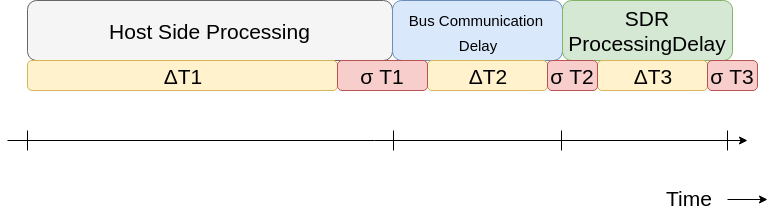
\includegraphics[width=0.75\textwidth]{Figure/RQ1.png}
\caption{Research Question}
\label{rq1}
\end{figure}

The research question is explained using Figure \ref{rq1}.
The Host Side processing delay is introduced by running the software implementation of the 802.15.4 \ac{PHY} and \ac{mac} layers.
The bus communication delay represents the delay caused by the \ac{USB} 3.0 bus transfers.
The \ac{sdr} processing delay is the time required by the LimeSDR platform for transmission or reception of radio signals.
The objective of this thesis is to quantitatively evaluate these delays and the impact of different network and \ac{sdr} configuration parameters.
%\item{ How to implement precise scheduling in LimeSDR based IEEE 802.15.4 communication system? }
%\end{itemize}

\section{Report Outline}
The remainder of the report is structured as follows. \textit{Chapter 2} introduces the relevant background information for understanding the rest of the report.
Relevant previous work will be introduced in \textit{Chapter 3}.
\textit{Chapter 4} introduces the experimental setup and the methods used in the measurement of the timing delays. \textit{Chapter 5} presents the experimental results and analysis.
The method used in mitigation of these delays will be introduced in \textit{Chapter 6}.
\textit{Chapter 7} presents the experimental results and analysis of the mitigation technique used.
Finally, \textit{Chapter 8} includes the concluding remarks and scope of future work.
